% \iffalse

\let\negmedspace\undefined
\let\negthickspace\undefined
\documentclass[journal,12pt,twocolumn]{IEEEtran}
\usepackage{cite}
\usepackage{amsmath,amssymb,amsfonts,amsthm}
\usepackage{algorithmic}
\usepackage{graphicx}
\usepackage{textcomp}
\usepackage{xcolor}
\usepackage{txfonts}
\usepackage{listings}
\usepackage{enumitem}
\usepackage{mathtools}
\usepackage{gensymb}
\usepackage{comment}
\usepackage[breaklinks=true]{hyperref}
\usepackage{tkz-euclide} 
\usepackage{listings}
\usepackage{gvv}                                        
\def\inputGnumericTable{}                                 
\usepackage[latin1]{inputenc}                                
\usepackage{color}                                            
\usepackage{array}                                            
\usepackage{longtable}                                       
\usepackage{calc}                                             
\usepackage{multirow}                                         
\usepackage{hhline}                                          
\usepackage{ifthen}                                           
\usepackage{lscape}
\usepackage{float}
\usepackage{adjustbox}

\newtheorem{theorem}{Theorem}[section]
\newtheorem{problem}{Problem}
\newtheorem{proposition}{Proposition}[section]
\newtheorem{lemma}{Lemma}[section]
\newtheorem{corollary}[theorem]{Corollary}
\newtheorem{example}{Example}[section]
\newtheorem{definition}[problem]{Definition}
\newcommand{\BEQA}{\begin{eqnarray}}
\newcommand{\EEQA}{\end{eqnarray}}
\newcommand{\define}{\stackrel{\triangle}{=}}
\theoremstyle{remark}
\parindent 0px
\newtheorem{rem}{Remark}
\begin{document}

\bibliographystyle{IEEEtran} 

\title{NCERT-12.8.7}
\author{\textbf{EE23BTECH11005} - Ambati Krishna Kaustubh% <-this % stops a space
}
\maketitle
\newpage
\bigskip

\renewcommand{\thefigure}{\arabic{figure}}
\renewcommand{\thetable}{\arabic{table}}
\section*{Question}

The amplitude  of the magnetic part of a harmonic elctromagnetic wave
is $B_0=510$nT.What is the amplitude of the electric part of the electromagnetic wave. 
   
\solution
%\fi
 \begin{align}\frac{E_0}{B_0}=c\end{align}
 \begin{align}
     E_0=c*B_0
 \end{align}
 \begin{align}E_0=153V-m\end{align}
 \begin{table}[H]
    \center

    \begin{tabular}{|c|c|c|}
    \hline
        \textbf{Parameter}&\textbf{Description}&\textbf{Value}\\
        \hline
        $B_0$&Amplitude of the Electric Field&510nT\\
        \hline
        $c$&Speed of Electro Magnetic Wave&$3 \times 10^8 ms^{-1}$ \\
        \hline
        $E_0$ &amplitude of the Electric Field&153V-m \\
        \hline
       \end{tabular} 
    \caption{Parameter Table}

    \label{tab:12.8.7}
\end{table}



Consider the general equation of Electric Field and Magnetic field
\begin{align}
    E=E_0\sin(\omega t-kx)
\end{align}
\begin{align}
    B=B_0\sin(\omega t-kx)
\end{align}
\begin{figure}[h]
    \centering
    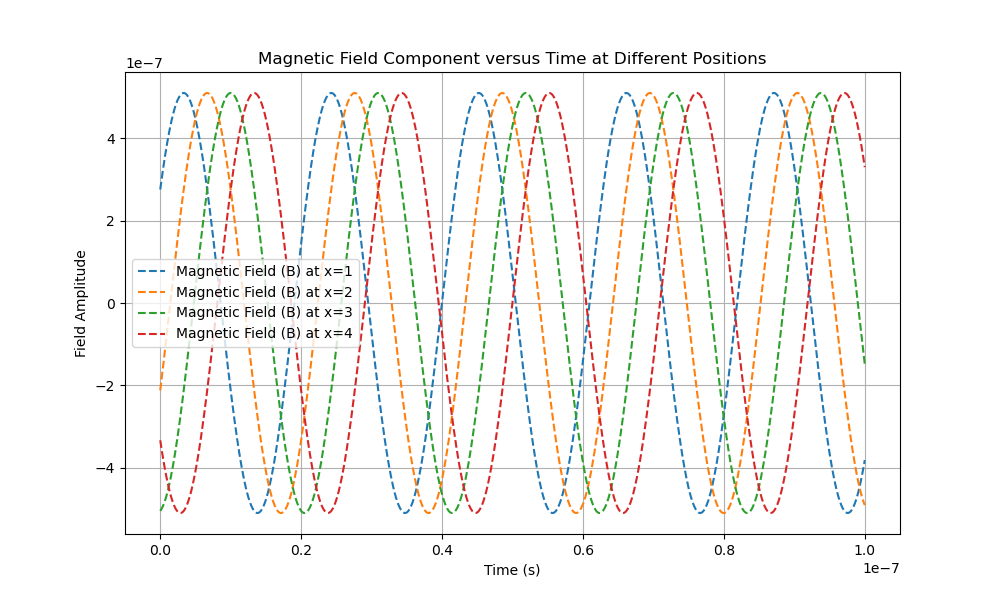
\includegraphics[width=\linewidth]{figs/analog1.png}
    \caption{Graph of Magnetic Field vs Time}
\end{figure}
\begin{figure}[h]
    \centering
    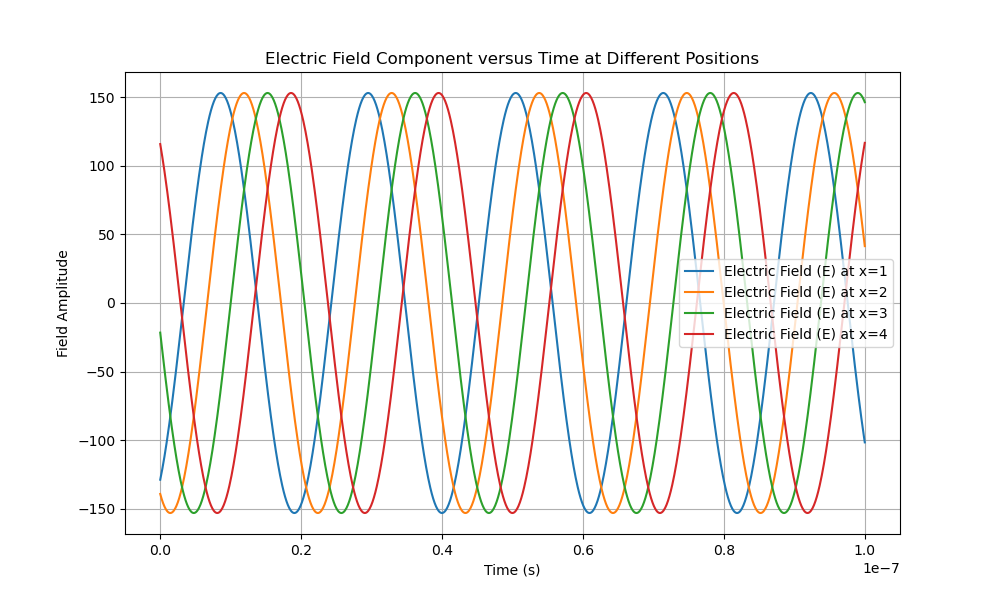
\includegraphics[width=\linewidth]{figs/analog2.png}
    \caption{Graph of Electric Field vs Time}
\end{figure}
\end{document}
